% Options for packages loaded elsewhere
\PassOptionsToPackage{unicode}{hyperref}
\PassOptionsToPackage{hyphens}{url}
\PassOptionsToPackage{dvipsnames,svgnames,x11names}{xcolor}
%
\documentclass[
  12pt]{article}

\usepackage{amsmath,amssymb}
\usepackage{iftex}
\ifPDFTeX
  \usepackage[T1]{fontenc}
  \usepackage[utf8]{inputenc}
  \usepackage{textcomp} % provide euro and other symbols
\else % if luatex or xetex
  \usepackage{unicode-math}
  \defaultfontfeatures{Scale=MatchLowercase}
  \defaultfontfeatures[\rmfamily]{Ligatures=TeX,Scale=1}
\fi
\usepackage{lmodern}
\ifPDFTeX\else  
    % xetex/luatex font selection
\fi
% Use upquote if available, for straight quotes in verbatim environments
\IfFileExists{upquote.sty}{\usepackage{upquote}}{}
\IfFileExists{microtype.sty}{% use microtype if available
  \usepackage[]{microtype}
  \UseMicrotypeSet[protrusion]{basicmath} % disable protrusion for tt fonts
}{}
\makeatletter
\@ifundefined{KOMAClassName}{% if non-KOMA class
  \IfFileExists{parskip.sty}{%
    \usepackage{parskip}
  }{% else
    \setlength{\parindent}{0pt}
    \setlength{\parskip}{6pt plus 2pt minus 1pt}}
}{% if KOMA class
  \KOMAoptions{parskip=half}}
\makeatother
\usepackage{xcolor}
\setlength{\emergencystretch}{3em} % prevent overfull lines
\setcounter{secnumdepth}{5}
% Make \paragraph and \subparagraph free-standing
\ifx\paragraph\undefined\else
  \let\oldparagraph\paragraph
  \renewcommand{\paragraph}[1]{\oldparagraph{#1}\mbox{}}
\fi
\ifx\subparagraph\undefined\else
  \let\oldsubparagraph\subparagraph
  \renewcommand{\subparagraph}[1]{\oldsubparagraph{#1}\mbox{}}
\fi


\providecommand{\tightlist}{%
  \setlength{\itemsep}{0pt}\setlength{\parskip}{0pt}}\usepackage{longtable,booktabs,array}
\usepackage{calc} % for calculating minipage widths
% Correct order of tables after \paragraph or \subparagraph
\usepackage{etoolbox}
\makeatletter
\patchcmd\longtable{\par}{\if@noskipsec\mbox{}\fi\par}{}{}
\makeatother
% Allow footnotes in longtable head/foot
\IfFileExists{footnotehyper.sty}{\usepackage{footnotehyper}}{\usepackage{footnote}}
\makesavenoteenv{longtable}
\usepackage{graphicx}
\makeatletter
\def\maxwidth{\ifdim\Gin@nat@width>\linewidth\linewidth\else\Gin@nat@width\fi}
\def\maxheight{\ifdim\Gin@nat@height>\textheight\textheight\else\Gin@nat@height\fi}
\makeatother
% Scale images if necessary, so that they will not overflow the page
% margins by default, and it is still possible to overwrite the defaults
% using explicit options in \includegraphics[width, height, ...]{}
\setkeys{Gin}{width=\maxwidth,height=\maxheight,keepaspectratio}
% Set default figure placement to htbp
\makeatletter
\def\fps@figure{htbp}
\makeatother

\addtolength{\oddsidemargin}{-.5in}%
\addtolength{\evensidemargin}{-1in}%
\addtolength{\textwidth}{1in}%
\addtolength{\textheight}{1.7in}%
\addtolength{\topmargin}{-1in}%
\usepackage{booktabs}
\usepackage{longtable}
\usepackage{array}
\usepackage{multirow}
\usepackage{wrapfig}
\usepackage{float}
\usepackage{colortbl}
\usepackage{pdflscape}
\usepackage{tabu}
\usepackage{threeparttable}
\usepackage{threeparttablex}
\usepackage[normalem]{ulem}
\usepackage{makecell}
\usepackage{xcolor}
\usepackage{amsmath}
\usepackage{float}
\usepackage{hyperref}
\usepackage[utf8]{inputenc}
\usepackage{bm}
\def\tightlist{}
\usepackage{setspace}
\newcommand\pD{$p\text{-}D$}
\newcommand\kD{$k\text{-}D$}
\newcommand\dD{$d\text{-}D$}
\newcommand\gD{$2\text{-}D$}
\makeatletter
\@ifpackageloaded{caption}{}{\usepackage{caption}}
\AtBeginDocument{%
\ifdefined\contentsname
  \renewcommand*\contentsname{Table of contents}
\else
  \newcommand\contentsname{Table of contents}
\fi
\ifdefined\listfigurename
  \renewcommand*\listfigurename{List of Figures}
\else
  \newcommand\listfigurename{List of Figures}
\fi
\ifdefined\listtablename
  \renewcommand*\listtablename{List of Tables}
\else
  \newcommand\listtablename{List of Tables}
\fi
\ifdefined\figurename
  \renewcommand*\figurename{Figure}
\else
  \newcommand\figurename{Figure}
\fi
\ifdefined\tablename
  \renewcommand*\tablename{Table}
\else
  \newcommand\tablename{Table}
\fi
}
\@ifpackageloaded{float}{}{\usepackage{float}}
\floatstyle{ruled}
\@ifundefined{c@chapter}{\newfloat{codelisting}{h}{lop}}{\newfloat{codelisting}{h}{lop}[chapter]}
\floatname{codelisting}{Listing}
\newcommand*\listoflistings{\listof{codelisting}{List of Listings}}
\makeatother
\makeatletter
\makeatother
\makeatletter
\@ifpackageloaded{caption}{}{\usepackage{caption}}
\@ifpackageloaded{subcaption}{}{\usepackage{subcaption}}
\makeatother
\ifLuaTeX
  \usepackage{selnolig}  % disable illegal ligatures
\fi
\usepackage[]{natbib}
\bibliographystyle{agsm}
\usepackage{bookmark}

\IfFileExists{xurl.sty}{\usepackage{xurl}}{} % add URL line breaks if available
\urlstyle{same} % disable monospaced font for URLs
\hypersetup{
  pdftitle={Looking at Non-Linear Dimension Reductions as Models in the Data Space},
  pdfauthor={Jayani P.G. Lakshika; Dianne Cook; Paul Harrison; Michael Lydeamore; Thiyanga S. Talagala},
  pdfkeywords={high-dimensional data, dimension reduction, hexagonal
binning, low-dimensional manifold, tour, data vizualization, model in
the data space},
  colorlinks=true,
  linkcolor={blue},
  filecolor={Maroon},
  citecolor={Blue},
  urlcolor={Blue},
  pdfcreator={LaTeX via pandoc}}


\begin{document}


\def\spacingset#1{\renewcommand{\baselinestretch}%
{#1}\small\normalsize} \spacingset{1}


%%%%%%%%%%%%%%%%%%%%%%%%%%%%%%%%%%%%%%%%%%%%%%%%%%%%%%%%%%%%%%%%%%%%%%%%%%%%%%

\title{\bf Looking at Non-Linear Dimension Reductions as Models in the
Data Space}
\author{
Jayani P.G. Lakshika\\
Econometrics \& Business Statistics, Monash University\\
and\\Dianne Cook\\
Econometrics \& Business Statistics, Monash University\\
and\\Paul Harrison\\
MGBP, BDInstitute, Monash University\\
and\\Michael Lydeamore\\
Econometrics \& Business Statistics, Monash University\\
and\\Thiyanga S. Talagala\\
Statistics, University of Sri Jayewardenepura\\
}
\maketitle

\bigskip
\bigskip
\begin{abstract}
Nonlinear dimension reduction (NLDR) techniques such as tSNE, and UMAP
provide a low-dimensional representation of high-dimensional (high-D)
data using non-linear transformation. The methods and parameter choices
can create wildly different representations, making it difficult to
decide which is best, or whether any or all are accurate or misleading.
NLDR often exaggerates random patterns, sometimes due to the samples
observed. But NLDR views have an important role in data analysis
because, if done well, they provide a concise visual (and conceptual)
summary of high-D distributions. To help evaluate the NLDR we have
developed an algorithm to show the 2D NLDR model in the high-D space,
viewed with a tour. One can see if the model fits everywhere or better
in some subspaces, or completely mismatches the data. It is used to
evaluate which 2D layout is the best representation of the high-D
distribution and see how different methods may have similar summaries or
quirks.
\end{abstract}

\noindent%
{\it Keywords:} high-dimensional data, dimension reduction, hexagonal
binning, low-dimensional manifold, tour, data vizualization, model in
the data space
\vfill

\newpage
\spacingset{1.9} % DON'T change the spacing!

\spacingset{1.0}

\section{Introduction}\label{introduction}

Non-linear dimension reduction (NLDR) is popular for making a convenient
low-dimensional (\kD{}) representation of high-dimensional (\pD{}) data.
Recently developed methods include t-distributed stochastic neighbor
embedding (tSNE) \citep{laurens2008}, uniform manifold approximation and
projection (UMAP) \citep{leland2018}, potential of heat-diffusion for
affinity-based trajectory embedding (PHATE) algorithm \citep{moon2019},
large-scale dimensionality reduction Using triplets (TriMAP)
\citep{amid2022}, and pairwise controlled manifold approximation
(PaCMAP) \citep{yingfan2021}. However, the representation generated can
vary dramatically from method to method, and with different choices of
parameters or random seeds made using the same method
(Figure~\ref{fig-NLDR-variety}). The dilemma for the analyst is then,
\textbf{which representation to use}. The choice might result in
different procedures used in the downstream analysis, or different
inferential conclusions. The research described here provides new visual
tools to aid with this decision.

\begin{figure}

\centering{

\includegraphics[width=1\textwidth,height=\textheight]{paper_files/figure-pdf/fig-NLDR-variety-1.pdf}

}

\caption{\label{fig-NLDR-variety}Six different NLDR representations of
the same data. Different techniques and different parameter choices are
used. Researchers may have seen any of these in their analysis of this
data, depending on their choice of method, or typical parameter choice.
Would they make different decisions downstream in the analysis depending
on which version seen? Which is the most accurate representation of the
structure in high dimensions?}

\end{figure}%

The paper is organised as follows. Section~\ref{sec-background} provides
a summary of the literature on NLDR, and high-dimensional data
visualization methods. Section~\ref{sec-method} contains the details of
the new methodology, including simulated data examples. Two applications
illustrating the use of the new methodology for bioinformatics and image
classification are in Section~\ref{sec-applications}. Limitations and
future directions are provided in Section~\ref{sec-discussion}.

\section{Background}\label{sec-background}

Historically, \kD{} representations of \pD{} data have been computed
using multidimensional scaling (MDS) \citep{borg2005}, which includes
principal components analysis (PCA) \citep{jolliffe2011} as a special
case. The \kD{} representation can be considered to be a layout of
points in \kD{} produced by an embedding procedure that maps the data
from \pD{}. In MDS, the \kD{} layout is constructed by minimizing a
stress function that differences distances between points in \pD{} with
potential distances between points in \kD{}. Various formulations of the
stress function result in non-metric scaling \citep{saeed2018} and
isomap \citep{silva2002}. Challenges in working with high-dimensional
data, including visualization, are outlined in \citet{johnstone2009}.

Many new methods for NLDR have emerged in recent years, all designed to
better capture specific structures potentially existing in \pD{}. Here
we focus on five currently popular techniques, tSNE, UMAP, PHATE, TriMAP
and PaCMAP. tNSE and UMAP can be considered to produce the \kD{}
minimizing the divergence between two distributions, where the
distributions are modeling the inter-point distances. PHATE, TriMAP and
PaCMAP are examples of diffusion processes \citep{coifman2005} spreading
to capture geometric shapes, that include both global and local
structure.

The array of layouts in Figure~\ref{fig-NLDR-variety} illustrate what
can emerge from the choices of method and parameters, and the random
seed that initiates the computation. Key structures interpreted from
these views suggest: (1) highly \textbf{separated clusters} (a, b, e, g,
h) with the number ranging from 3-6; (2) \textbf{stringy branches} (f),
and (3) \textbf{barely separated clusters} (c, d) which would
\textbf{contradict} the other representations.

It happens because these methods and parameter choices provide different
lenses on the interpoint distances in the data.

The alternative approach to visualizing the high-dimensional data is to
use linear projections. PCA is the classical approach, resulting in a
set of new variables which are linear combinations of the original
variables. Tours, defined by \citet{lee2021}, broaden the scope by
providing movies of linear projections, that provide views the data from
all directions. \citet{lee2021} provides an review of the main
developments in tours. There are many tour algorithms implemented, with
many available in the R package \texttt{tourr} \citep{wickham2011}, and
versions enabling better interactivity in \texttt{langevitour}
\citep{harisson2024} and \texttt{detourr} \citep{hart2022}. Linear
projections are a safe way to view high-dimensional data, because they
do not warp the space, so they are more faithful representations of the
structure. However, linear projections can be cluttered, and global
patterns can obscure local structure. The simple activity of projecting
data from \pD{} suffers from piling \citep{laa2022}, where data
concentrates in the center of projections. NLDR is designed to escape
these issues, to exaggerate structure so that it can be observed. But as
a result NLDR can hallucinate wildly, to suggest patterns that are not
actually present in the data.

The solution is to use the tour to examine how the NLDR is warping the
space. This approach follows what \citet{wickham2015} describes as
\emph{model-in-the-data-space}. The fitted model should be overlaid on
the data, to examine the fit relative the spread of the observations.
While this is straightforward, and commonly done when data is 2D, it is
also possible in \pD{}, for many models, when a tour is used.

\citet{wickham2015} provides several examples of models overlaid on the
data in \pD{}. In hierarchical clustering, a representation of the
dendrogrom using points and lines can be constructed by augmenting the
data with points marking merging of clusters. Showing the movie of
linear projections reveals shows how the algorithm sequentially fitted
the cluster model to the data. For linear discriminant analysis or
model-based clustering the model can be indicated by \((p-1)\text{-}D\)
ellipses. It is possible to see whether the elliptical shapes
appropriately matches the variance of the relevant clusters, and to
compare and contrast different fits. For PCA, one can display the \kD{}
plane of the reduced dimension using wireframes of transformed cubes.
Using a wireframe is the approach we take here, to represent the NLDR
model in \pD{}.

\section{Method}\label{sec-method}

\subsection{What is the NLDR model?}\label{what-is-the-nldr-model}

At first glance, thinking of NLDR as a modeling technique might seem
strange. It is a simplified representation or abstraction of a system,
process, or phenomenon in the real world. The \pD{} observations are the
realization of the phenomenon, and the \kD{} NLDR layout is the
simplified representation. From a statistical perspective we can
consider the distances between points in the \kD{} layout to be variance
that the model explains, and the (relative) difference with their
distances in \pD{} is the error, or unexplained variance. We can also
imagine that the positioning of points in 2D represent the fitted
values, that will have some prescribed position in \pD{} that can be
compared with their observed values. This is the conceptual framework
underlying the more formal versions of factor analysis \citep{cfa69} and
multidimensional scaling (MDS) \citep{borg2005}. (Note that, for this
thinking the full \pD{} data needs to be available, not just the
interpoint distances.)

\begin{table}

\centering{

\centering\begingroup\fontsize{12}{14}\selectfont

\begin{tabular}{>{\raggedright\arraybackslash}p{3cm}>{\raggedright\arraybackslash}p{12cm}}
\toprule
\textbf{Notation} & \textbf{Description}\\
\midrule
$n, p, k, m$ & number of observations, variables, embedding dimension, number of non-empty bins, respectively\\
$\mathbfit{X}, \mathbfit{x}$ & $p$-dimensional data (population, sample)\\
$\mathbfit{y}$ & $k$-dimensional layout\\
$P$ & orthonormal basis, generating a $d\text{-}dimensional$ linear projection of $p$-dimensional data\\
$T$ & true  model\\
\addlinespace
$g$ & functional mapping from \pD{} to \kD{}, especially as prescribed by NLDR\\
$\mathbfit{\theta}$ & (Hyper-) parameters for NLDR method\\
$r$ & ranges of the embedding components\\
$C^{(j)}$ & $j$-dimensional bin centers\\
$(b_1, b_2)$ & number of bins in each direction\\
\addlinespace
$(a_1, a_2)$ & binwidths, distance between centroids in each direction\\
$(s_1, \ s_2)$ & starting coordinates of the hexagonal grid\\
$q$ & buffer to ensure hexgrid covers data, proportion of data range, 0-1\\
$b$, $b'$ & total and non-empty hexagon bins in the grid\\
$n_k$ & number of observations within the $k^{th}$ hexagon\\
\bottomrule
\end{tabular}
\endgroup{}

}

\caption{\label{tbl-notation}Summary of notation for describing new
methodology.}

\end{table}%

We define the NLDR as a function
\(g\text{:}~ \mathbb{R}^{n\times p} \rightarrow \mathbb{R}^{n\times k}\),
with (hyper-)parameters \(\mathbfit{\theta}\). The parameters,
\(\mathbfit{\theta}\), depend on the choice of \(g\), and can be
considered part of model fitting in the traditional sense. Common
choices for \(g\) include functions used in tSNE, UMAP, PHATE, TriMAP,
PaCMAP, or MDS, although in theory any function that does this mapping
is suitable.

With our goal being to make a representation of this 2D layout that can
be lifted into high-dimensional space, the layout needs to be augmented
to include neighbour information. A simple approach would be to
triangulate the points and add edges. A more stable approach is to first
hexagonally bin the data, reducing it from \(n\) to \(m\leq n\)
observations, and connect the bin centroids. This process serves to
reduce some noisiness in the resulting surface shown in \pD{}. The steps
in this process are shown in Figure~\ref{fig-NLDR-scurve}, and
documented below.

\begin{figure}

\centering{

\includegraphics[width=1\textwidth,height=\textheight]{paper_files/figure-pdf/fig-NLDR-scurve-1.pdf}

}

\caption{\label{fig-NLDR-scurve}Key steps for constructing the model on
the UMAP layout (\(k=2\)) of the S-curve data: (a) data, (b) hexagon
bins, (c) bin centroids, and (d) triangulated centroids.}

\end{figure}%

To illustrate the method, we use \(7\text{-}D\) simulated data, which we
call the ``S-curve''. It is constructed by setting
\(X_1 = \sin(a), X_2 = U(0, 2), X_3 = \text{sign}(a) \times (\cos(a) - 1), \forall a \in [-3\pi/2, 3\pi/2]\).
The remaining variables \(X_4, X_5, X_6, X_7\) are all uniform error,
with small variance. We would consider \(T=(X_1, X_2, X_3)\) to be the
true model.

\subsubsection{Scaling the data}\label{scaling-the-data}

It is beneficial to define the algorithm on data having a standard
scale. Here the variables are scaled to {[}0, 1{]}, but the upper bound
can incorporate the aspect ratio produced by the NLDR
\((r_1, r_2, ..., r_k)\), by setting them to
\((y_{1,\text{max}}, y_{2,\text{max}}, ..., y_{k,\text{max}})\). When
\(k=2\) which is assumed for hexagon binning, \(y_{1,\text{max}}=1\) and
\(y_{2,\text{max}} = \frac{r_2}{r_1}\), as observed in
Figure~\ref{fig-NLDR-scurve}.

\subsubsection{Computing hexagon grid
configurations}\label{computing-hexagon-grid-configurations}

The 2D hexagon grid is defined by the number of bins in each direction
\((b_1, b_2)\), giving total number of bins as \(b = b_1 \times b_2\),
and hexagon id, \(h = 1, \dots, b\). Each hexagon, \(H_h\) is uniquely
described by centroid, \$ C\_\{h\}\^{}\{(2)\} = (c\_\{h1\},
c\_\{h2\})\$. The lower left position where the grid starts at
\((s_1, s_2)\), which correspond to the lowest left centroid. The values
of \(s_i\) need to be below their respective minimum variable values,
and could be a full bin lower, to allow a buffer (\(q\)) corresponding
to a full hexagon width (\(a_1\)) and height (\(a_2\)) around the data.
The values of \(b_i\) are variables to be computed that define the
reduction in size of the data (\(n\) to \(m\)).

The value for \(b_2\) is computed by fixing \(b_1\). Considering the
lower bound of the NLDR, \(a_1 > -2q\), and
\(a_1 > \frac{1+q}{b_1 -1}\). Similarly, according to the upper bound of
the NLDR, \(a_1 > \frac{2r_2(1 + q)}{\sqrt{3}(b_2 - 1)}\), because
\(a_2 = \frac{\sqrt(3)}{2}a_1\) for regular hexagons. Therefore,
\(b_2 = \Big\lceil1 +\frac{2r_2(b_1 - 1)}{\sqrt{3}}\Big\rceil\).

\begin{figure}[H]

\centering{

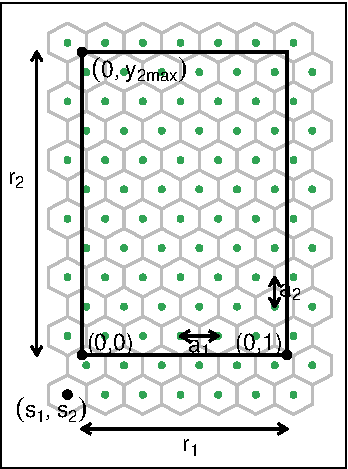
\includegraphics[width=1\textwidth,height=0.3\textheight]{paper_files/figure-pdf/fig-hex-param-1.pdf}

}

\caption{\label{fig-hex-param}Notations for hexagonal grid
configurations.}

\end{figure}%

\subsubsection{Binning the data}\label{binning-the-data}

Points are allocated to the bin they fall into based on the nearest
centroid. In situations where a point is equidistant from multiple
centroids, tie-breaking rules are applied. If multiple centroids are in
the same row, the point is assigned to the leftmost centroid. If
multiple centroids are in different rows, the point is assigned to the
bottom centroid.

\(\{ i \in H_h, h = 1, \dots, b, \text{ and } i = 1, \dots, n\}\)

\subsubsection{Summarization of the data in
2D}\label{summarization-of-the-data-in-2d}

Let \(h : \mathbb{R}^{n\times k} \rightarrow \mathbb{R}^{m\times k}\) be
the function that maps a point in \kD{} space to it's bin centroid
(\(C^{(k)}\)). This is the model points in \kD{} space.

When \(k = 2\), one of the representations of a bin is the hexagonal
centroid (Figure~\ref{fig-NLDR-scurve} (c)).

\subsubsection{Generating edges to indicate neighbours and removing long
edges}\label{generating-edges-to-indicate-neighbours-and-removing-long-edges}

Delaunay triangulation is used to connect neighbouring centroids, which
is needed to preserve neighbourhood information when the model is lifted
into \pD{}.

When \(k = 2\) Delaunay triangulation on \(C^{(2)}\) generates the model
in 2D space, which is a triangular mesh (Figure~\ref{fig-NLDR-scurve}
(d)). It generates convex hulls of \(C^{(2)}\) such that the
circumcircle of every triangle in the triangulation contains no other
points from \(C^{(2)}\).

\subsection{\texorpdfstring{Displaying the model in
\pD{}}{Displaying the model in }}\label{displaying-the-model-in}

The last step is to lift the \kD{} model into \pD{} by computing \pD{}
vectors that represent bin centroids. Define the set \(H^k\) to be the
set of points that belong to bin \(k\). We use the \pD{} Euclidean mean
of the points in \(H^k\) to map the centroid \((h_x^k, h_y^k)\) to a
point in \pD{}. Let the \(i\)-th component of the \pD{} mean be

\[f_i = \frac{1}{\left|H^k\right|}\sum_{y \in H^k} y_i,\]

with corresponding \pD{} vector \(\vec{f_i}\). Then, \(f(h\circ g)(x)\)
maps a \pD{} point to the \pD{} model estimate, completing the model
cycle.

Furthermore, edges that exist between \kD{} representations should also
generate edges in \pD{} by connecting \pD{} mapping of the corresponding
\kD{} representations.

\subsection{Measuring the fit}\label{sec-summary}

\subsubsection{Fitted values}\label{fitted-values}

The prediction approach involves performing the K-nearest neighbors
(KNN) algorithm for an unsupervised classification problem. First, the
nearest high-D model point is identified for a given new high-D point.
Then, the corresponding 2D centroid mapping for the identified high-D
model point is determined. Finally, the coordinates of this 2D centroid
are used as the predicted 2D embedding for the new high-D data point.
This step is particularly valuable due to the limitations of some NLDR
techniques, like tSNE, which don't provide a straightforward method for
prediction. As a result, our approach offers a solution that capable of
generating predicted 2D embedding regardless of the NLDR technique
employed, effectively addressing this functional gap.

\subsubsection{Error calculation}\label{error-calculation}

Residuals are essential for evaluating the accuracy of representing
high-D points by the high-D mapping of 2D bin centroids. To measure this
accuracy, an error metric is introduced, quantifying the sum of squared
differences between the high-D data (\(x_{ij}\)) and the high-D mapping
of the 2D bin centroid data (\(C_{x_ij}\)) across all observations and
dimensions (see Equation~\ref{eq-equation10}).

\begin{equation}\phantomsection\label{eq-equation10}{
\text{Error} = \sum_{j = 1}^{n}\sum_{i = 1}^{p} (x_{ij} - C_{x_ij})^2
}\end{equation}

Here, \(n\) represents the number of observations, \(p\) represents the
dimensions of high-D data, \(x_{ij}\) is the high-D data, and
\(C_{x_ij}\) is the high-D mapping of the 2D bin centroid.

To assess how well our method captures and represents the underlying
structure of the high-D data, Mean Squared Error (MSE) is used. When
computing MSE, total model error (see Section~\ref{sec-summary}) is
divided by the number of observations to make it as a mean value (see
Equation~\ref{eq-equation9}).

\begin{equation}\phantomsection\label{eq-equation9}{
\text{MSE} = \sum_{j = 1}^{n} \frac{\sum_{i = 1}^{p} (x_{ij} - C_{x_ij})^2}{n}
}\end{equation}

\subsection{Tuning}\label{tuning}

The performance and robustness of our model depend on three key
parameters: (i) the total number of bins (\(b\)), (ii) a benchmark value
used to remove low-density hexagons, and (iii) a benchmark value used to
remove long edges. However, there is no analytical formula to calculate
an appropriate value for these parameters. The selection of these
parameter values depends on the model performance computed by MSE (see
Section~\ref{sec-summary}).

\subsubsection{Choice of bins}\label{choice-of-bins}

The number of hexagonal bins in the hexagonal grid has a considerable
impact on the construction of the \gD{} model, serving as the initial
step. The chosen total number of bins must effectively capture the
structure of the NLDR data. If the number of bins is too low, the model
may not be able to capture the structure of the NLDR data effectively
(see Figure~\ref{fig-bins-scurve} (a)), while if there are too many
bins, it may result in over-fitting the individual points of the NLDR
data (see Figure~\ref{fig-bins-scurve} (c)). Therefore, it is important
to determine an effective number of bins to construct a reasonable model
(see Figure~\ref{fig-bins-scurve} (b)).

\begin{figure}[H]

\centering{

\includegraphics[width=1\textwidth,height=\textheight]{paper_files/figure-pdf/fig-bins-scurve-1.pdf}

}

\caption{\label{fig-bins-scurve}Hexbin plots from different number of
bins for the UMAP applied to S-curve data: (a) \(b = 12\) (3, 5), (b)
\(b = 190\) (10, 19), and (c) \(b = 2176\) (34, 64). The hexbins are
colored based on the density of points, with darker colors indicating
higher density and yellow color representing lower density within each
bin. What is the number of bins that would be effective?}

\end{figure}%

Furthermore, the total number of bins is calculated based on the number
of bins along the x-axis and y-axis, \(b = b_1 \times b_2\). To
determine the effective \(b\), candidate values are selected based on
the range between the minimum and approximate maximum \(b_1\), because
\(b_2\) is computed from \(b_1\). The minimum \(b_1\) is set to \(2\),
while the maximum number is estimated by taking the square root of
\(n\). The analysis evaluates the MSE across varying \(b\) within this
range, covering the minimum to maximum values along both axes (see
Figure~\ref{fig-mse-scurve-b}).

\begin{figure}[H]

\centering{

\includegraphics[width=1\textwidth,height=0.3\textheight]{paper_files/figure-pdf/fig-mse-scurve-b-1.pdf}

}

\caption{\label{fig-mse-scurve-b}MSE from UMAP applied to S-curve
dataset with diffferent \(b\) choices. What is the effective \(b\) to
create the model? The residual plot have a steep slope at the beginning,
indicating that a smaller \(b\) causes a larger amount of MSE. Then, the
slope gradually declines or level off, indicating that a higher \(b\)
generates a smaller MSE. Using the elbow method, it was observed that
when the \(b\) is set to \(190\), the lowest MSE occurred.}

\end{figure}%

\subsubsection{Removal of low density
bins}\label{removal-of-low-density-bins}

After establishing the hexagonal grid with an appropriate number of
bins, some hexagonal bins may have few or no data points within them
(see \textbf{?@fig-rmlowdenshex} (a)). To ensure comprehensive coverage
of the NLDR data, it is necessary to select hexagonal bins with a
considerable number of data points. This involves calculating the number
of points within each hexagon. Then, the standard count is computed by
dividing the number of points within each hexagon by the maximum number
of points in the grid (see \textbf{?@eq-equationp2}). Next, bins with a
standard count less than a certain benchmark value are removed (see
\textbf{?@fig-rmlowdenshex} (b)). The following steps will help in
determining a suitable value for removing low-density hexagons:

\begin{enumerate}
\def\labelenumi{\arabic{enumi}.}
\tightlist
\item
  Plot the distribution of the standardized counts (see
  \textbf{?@fig-stdctsScurve}).
\item
  Examine the distribution of counts.
\item
  Select the first quantile value if the distribution is skewed.
\end{enumerate}

\begin{figure}[H]

\centering{

\includegraphics[width=1\textwidth,height=0.5\textheight]{paper_files/figure-pdf/fig-stdcts-scurve-1.pdf}

}

\caption{\label{fig-stdcts-scurve}Distribution of standardize counts by
hexagons.}

\end{figure}%

Furthermore, selecting the benchmark value for removing low-density
hexagons is important. Removing unnecessary bins may lead to the
formation of long edges and an uneven 2D model. Hence, rather than
solely relying on the benchmark value to identify hexagons for removal,
it's essential to consider the standard number of points in the
neighboring hexagons of the identified low-density ones (see
\textbf{?@fig-rmlowdenshex} (c)). If neighboring bins also show low
counts, only those bins will be removed. The remaining bins are used to
construct the 2D model.

The benchmark value for removing low-density hexagons ranges between
\(0\) and \(1\). When analyzing how these benchmark values influence
model performance, it's essential to observe the change in MSE as the
benchmark value increases (see \textbf{?@fig-diagnosticpltScurvelwd}).
The MSE shows a gradual increase as the benchmark value progresses from
\(0\) to \(1\). Evaluating this rate of increase is important. If the
increment is not considerable, the decision might lean towards retaining
low-density hexagons.

\begin{figure}[H]

\centering{

\includegraphics[width=1\textwidth,height=0.5\textheight]{paper_files/figure-pdf/fig-mse-scurve-lwd-1.pdf}

}

\caption{\label{fig-mse-scurve-lwd}MSE from UMAP applied to S-curve
dataset with diffferent bechmark choices. What is the effective bechmark
value to remove low density hexagons? The residual plot have a steep
slope at the beginning, indicating that a smaller bechmark value causes
a larger amount of MSE. Then, the slope gradually declines or level off,
indicating that a higher bechmark value generates a smaller MSE. Using
the elbow method, it was observed that when the bechmark value is set to
\(0.6\), the lowest MSE occurred.}

\end{figure}%

\subsubsection{Removing long edges}\label{removing-long-edges}

Creating a smooth 2D representation (see \textbf{?@fig-modelScurve} (c))
requires removing edges that connect distant bin centroids within the
triangular mesh (see \textbf{?@fig-modelScurve} (b)). These edges only
exist in the 2D model and do not extend into higher dimensions, ensuring
that their removal does not impact the model in higher dimensions. While
specific criteria for determining the benchmark value to remove long
edges do not exist, the following steps provide an approach to
identifying a suitable threshold:

\begin{enumerate}
\def\labelenumi{\arabic{enumi}.}
\tightlist
\item
  Plot the distribution of the 2D Euclidean distances (see
  \textbf{?@fig-distScurve}).
\item
  Identify the largest difference between consecutive distance values.
\item
  Take the largest distance value corresponding to this difference as
  the benchmark value.
\end{enumerate}

\begin{figure}[H]

\centering{

\includegraphics[width=1\textwidth,height=0.5\textheight]{paper_files/figure-pdf/fig-dist-scurve-1.pdf}

}

\caption{\label{fig-dist-scurve}Distribution of \(2\text{-}D\) Euclidean
distances between bin centroids of the triangular mesh generated with
S-curve UMAP data.}

\end{figure}%

\subsection{Illustration on simulated
data}\label{illustration-on-simulated-data}

In this section, the effectiveness of the algorithm is described using a
simulated dataset. The dataset consists of five spherical Gaussian
clusters in \(4\text{-}D\), with each cluster containing an equal number
of points and the same within-cluster variation.

In the 2D layouts generated by various NLDR techniques, as shown in
Figure~\ref{fig-NLDR-variety-gau}, five well-separated clusters are
shown. In tSNE (see Figure~\ref{fig-NLDR-variety-gau} (a)), these
clusters appear closely. UMAP arranges all clusters in a parallel
manner, with three aligned in one line and the other two in a separate
line (see Figure~\ref{fig-NLDR-variety-gau} (b)). In contrast, PHATE
shows two closely positioned clusters and three more distant ones (see
Figure~\ref{fig-NLDR-variety-gau} (c)). In TriMAP, two clusters are
close, though not as tightly as PHATE, while the other three are
well-separated (see Figure~\ref{fig-NLDR-variety-gau} (d)). Finally,
PaCMAP shows one central cluster and the remaining four spread out in
different directions (see Figure~\ref{fig-NLDR-variety-gau} (e)).

\begin{figure}[H]

\centering{

\includegraphics[width=1\textwidth,height=\textheight]{paper_files/figure-pdf/fig-NLDR-variety-gau-1.pdf}

}

\caption{\label{fig-NLDR-variety-gau}Five different NLDR representations
of the same data. Different techniques and different parameter choices
are used. Is there a best representation of the original data or are
they all providing equivalent information?}

\end{figure}%

To investigate which is the reasonable representation to visualize the
five spherical Gaussian cluster data or all NLDR methods provide
equivalent information, we visualize all the models in \pD{} space.
Models from tSNE, UMAP, and PHATE show five well-separated clusters (see
\textbf{?@fig-gau1\_sc}, \textbf{?@fig-gau2\_sc}, and
\textbf{?@fig-gau3\_sc}), while PaCMAP and TriMAP have a long edge that
connects neighboring two clusters and three well-separated clusters (see
\textbf{?@fig-gau4\_sc}, and \textbf{?@fig-gau5\_sc}). This suggests
that for the five Gaussian cluster dataset, all NLDR methods effectively
preserve the global structure.

Models from all NLDR methods show five well-separated clusters (see
\textbf{?@fig-gau1\_sc}, \textbf{?@fig-gau2\_sc},
\textbf{?@fig-gau3\_sc}, \textbf{?@fig-gau4\_sc}, and
\textbf{?@fig-gau5\_sc}). This suggests that for the five Gaussian
cluster dataset, all NLDR methods effectively preserve the global
structure. tSNE, UMAP, and PHATE display clusters with varying
densities, indicating their ability to capture within-cluster variation
(see \textbf{?@fig-gau1\_sc}, \textbf{?@fig-gau2\_sc}, and
\textbf{?@fig-gau3\_sc}). On the other hand, both TriMAP and PaCMAP show
clusters with flat surfaces, suggesting a failure to capture
within-cluster variation (see \textbf{?@fig-gau4\_sc} and
\textbf{?@fig-gau5\_sc}). Therefore, TriMAP and PaCMAP do not capture
the local structure as effectively as other methods.

When compare the NLDR representations and generates models, tSNE with
perplexity \(61\) is the reasonable representation to visualize the five
Gaussian cluster dataset.

\begin{figure}[H]

\centering{

\includegraphics[width=1\textwidth,height=\textheight]{paper_files/figure-pdf/fig-trimesh-gau-1.pdf}

}

\caption{\label{fig-trimesh-gau}Model generated with five diiferent NLDR
methods in \(2\text{-}D\) with approximately \(65\) non-empty bins.}

\end{figure}%

\section{Applications}\label{sec-applications}

\subsection{pbmc}\label{pbmc}

In the field of single-cell studies, a common analytical task involves
clustering to identify groups of cells with similar expression profiles.
Analysts often turn to NLDR techniques to verify and identify these
clusters and explore developmental trajectories. To illustrate the
importance of NLDR techniques and parameter selection in identifying
clusters, Human Peripheral Blood Mononclear Cells (PBMC3k) dataset
\citep{chen2023} is used. In a study by \citet{chen2023}, this dataset
was used to demonstrate how UMAP represents clusters (see
Figure~\ref{fig-umap-author}). As shown in Figure~\ref{fig-umap-author},
there are three distinct and well-separated clusters.

\begin{figure}[H]

\centering{

\includegraphics[width=1\textwidth,height=0.3\textheight]{paper_files/figure-pdf/fig-umap-author-1.pdf}

}

\caption{\label{fig-umap-author}\(2\text{-}D\) layout from UMAP applied
for the PBMC3k dataset. Is this a best representation of the original
data? The parameter setting is n\_neighbors = 30, min\_dist = 0.3.}

\end{figure}%

To determine whether the UMAP representation with the parameter choice
suggested by \citet{chen2023} preserves the original data structure, we
visualize the model constructed with UMAP overlaid on the \pD{} data.
The figures in Figure~\ref{fig-pbmc1_sc} show three well-separated
clusters, indicating that the suggested UMAP representation preserves
the global structure (see Figure~\ref{fig-umap-author}). However, as
shown in Figure~\ref{fig-pbmc1_sc}, these clusters are close to each
other in \pD{}. Also, non-linear continuity patterns and high-density
patches within the clusters are observed (see
Figure~\ref{fig-pbmc1_sc}). Therefore, the suggested UMAP representation
(see Figure~\ref{fig-umap-author}) does not accurately preserve the
local structure of the PBMC3k dataset.

\begin{figure}[H]

\centering{

\includegraphics[width=1\textwidth,height=\textheight]{paper_files/figure-pdf/fig-model-pbmc-author-1.pdf}

}

\caption{\label{fig-model-pbmc-author}(a) Model generated in
\(2\text{-}D\) with UMAP, and (b) \(p\text{-}D\) model error in
\(2\text{-}D\). The \(2\text{-}D\) model shows three well-separated
distinct clusters. The \(p\text{-}D\) model errors are distributed along
clusters.}

\end{figure}%

\begin{figure}[H]

\begin{minipage}{0.33\linewidth}

\centering{

\captionsetup{labelsep=none}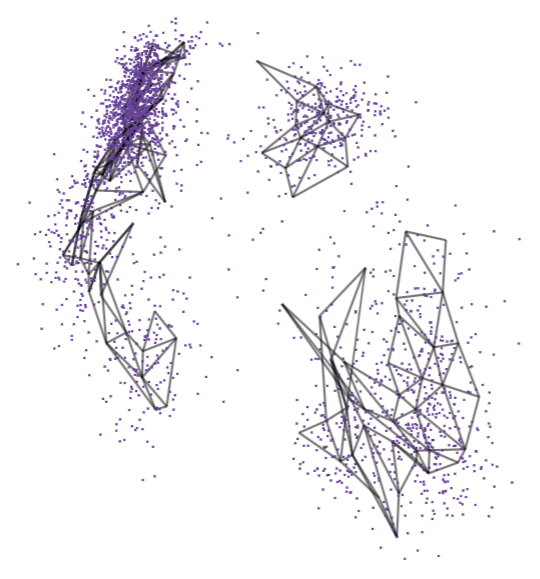
\includegraphics{figures/pbmc3k/sc_1.png}

}

\subcaption{\label{fig-pbmc1_sc1}}

\end{minipage}%
%
\begin{minipage}{0.33\linewidth}

\centering{

\captionsetup{labelsep=none}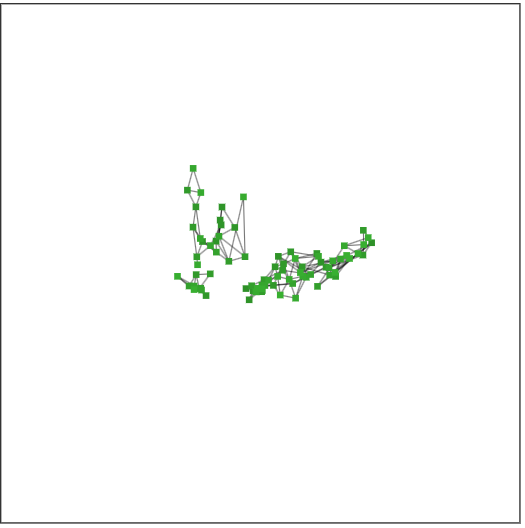
\includegraphics{figures/pbmc3k/sc_2.png}

}

\subcaption{\label{fig-pbmc1_sc2}}

\end{minipage}%
%
\begin{minipage}{0.33\linewidth}

\centering{

\captionsetup{labelsep=none}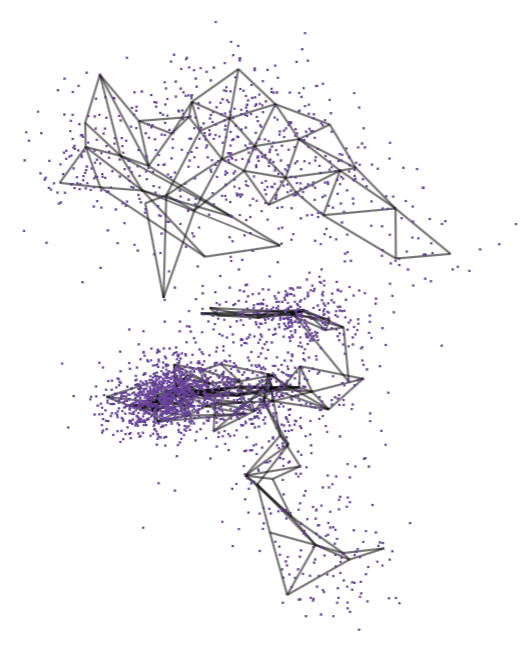
\includegraphics{figures/pbmc3k/sc_3.png}

}

\subcaption{\label{fig-pbmc1_sc3}}

\end{minipage}%

\caption{\label{fig-pbmc1_sc}Screen shots of the \textbf{langevitour} of
the PBMC3k data set, shows the model-in-data space, a video of the tour
animation is available at (\url{https://youtu.be/Gnhh4hfsbbg}).}

\end{figure}%

In order to find a reasonable NLDR representation for the PBMC3k
dataset, we calculated the absolute error for different numbers of
non-empty bins using various NLDR techniques and different parameter
settings (see Figure~\ref{fig-pbmc-abserror}). After analyzing the
results, we found that tSNE with a perplexity set to \(30\) had the
lowest error when the number of non-empty bins was \(137\). Therefore,
tSNE with a perplexity of \(30\), which is the default parameter
setting, is considered as a reasonable representation for the PBMC3k
dataset.

\begin{figure}[H]

\centering{

\includegraphics[width=0.5\textwidth,height=\textheight]{paper_files/figure-pdf/fig-pbmc-abserror-1.pdf}

}

\caption{\label{fig-pbmc-abserror}Absolute error from UMAP and tSNE
applied to training PBMC3k dataset with diffferent parameter choices.
What is the best parameter choice to create the model? The residual plot
have a steep slope at the beginning, indicating that a smaller number of
non-empty bins causes a larger amount of error. Then, the slope
gradually declines or level off, indicating that a higher number of
non-empty bins generates a smaller error. Using the elbow method, it was
observed that when the number of non-empty bins is set to \(137\), the
lowest error occurred with the parameters perplexity: \(30\).}

\end{figure}%

As shown in Figure~\ref{fig-tsne-suggest}, there are three
well-separated clusters, although they are located close to each other.
Additionally, non-linear structures can also be observed within the
clusters (see Figure~\ref{fig-model-pbmc} (a)). In this manner, tSNE was
able to capture the data structure for the PBMC3k dataset that UMAP
failed to do.

\begin{figure}[H]

\centering{

\includegraphics[width=0.4\textwidth,height=\textheight]{paper_files/figure-pdf/fig-tsne-suggest-1.pdf}

}

\caption{\label{fig-tsne-suggest}\(2\text{-}D\) layout from tSNE applied
for the PBMC3k dataset. Is this a best representation of the original
data? The parameter setting is perplexity=30.}

\end{figure}%

We then fit the model for tSNE, and visualize the resultant model in the
\pD{} data space. The model shows a quirk, as shown in
Figure~\ref{fig-pbmc2_sc}. All three clusters are connected by an edge
except the small and large clusters. Because the clusters are so close
in \gD{}, they attempt to maintain the structure in \pD{} as well. This
is evident that tSNE with perplexity \(30\) provides a reasonable
representation of PBMC3k data.

\begin{figure}[H]

\centering{

\includegraphics[width=1\textwidth,height=0.3\textheight]{paper_files/figure-pdf/fig-model-pbmc-1.pdf}

}

\caption{\label{fig-model-pbmc}(a) Model generated in \(2\text{-}D\)
with tSNE, and (b) \(p\text{-}D\) model error in \(2\text{-}D\). The
\(2\text{-}D\) model shows three well-separated distinct clusters. The
\(p\text{-}D\) model errors are distributed along clusters, but most low
\(p\text{-}D\) model errors present in the large cluster.}

\end{figure}%

\begin{figure}[H]

\begin{minipage}{0.33\linewidth}

\centering{

\captionsetup{labelsep=none}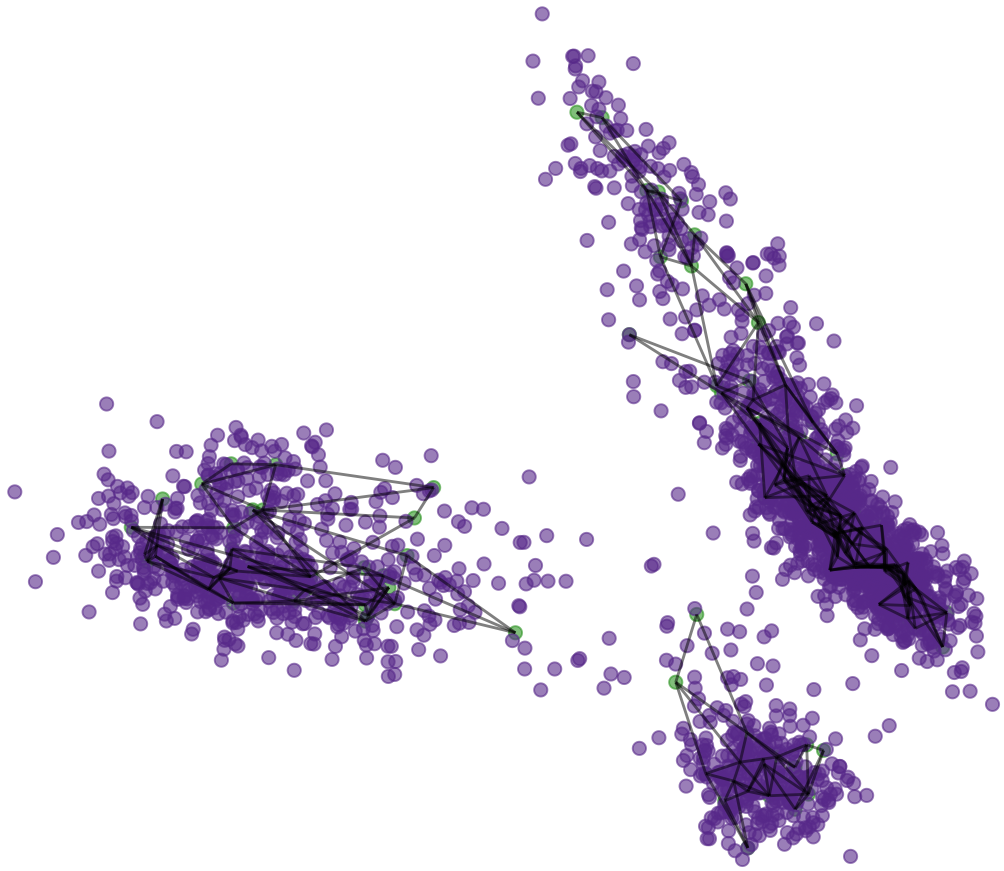
\includegraphics{figures/pbmc3k/sc_4.png}

}

\subcaption{\label{fig-pbmc2_sc4}}

\end{minipage}%
%
\begin{minipage}{0.33\linewidth}

\centering{

\captionsetup{labelsep=none}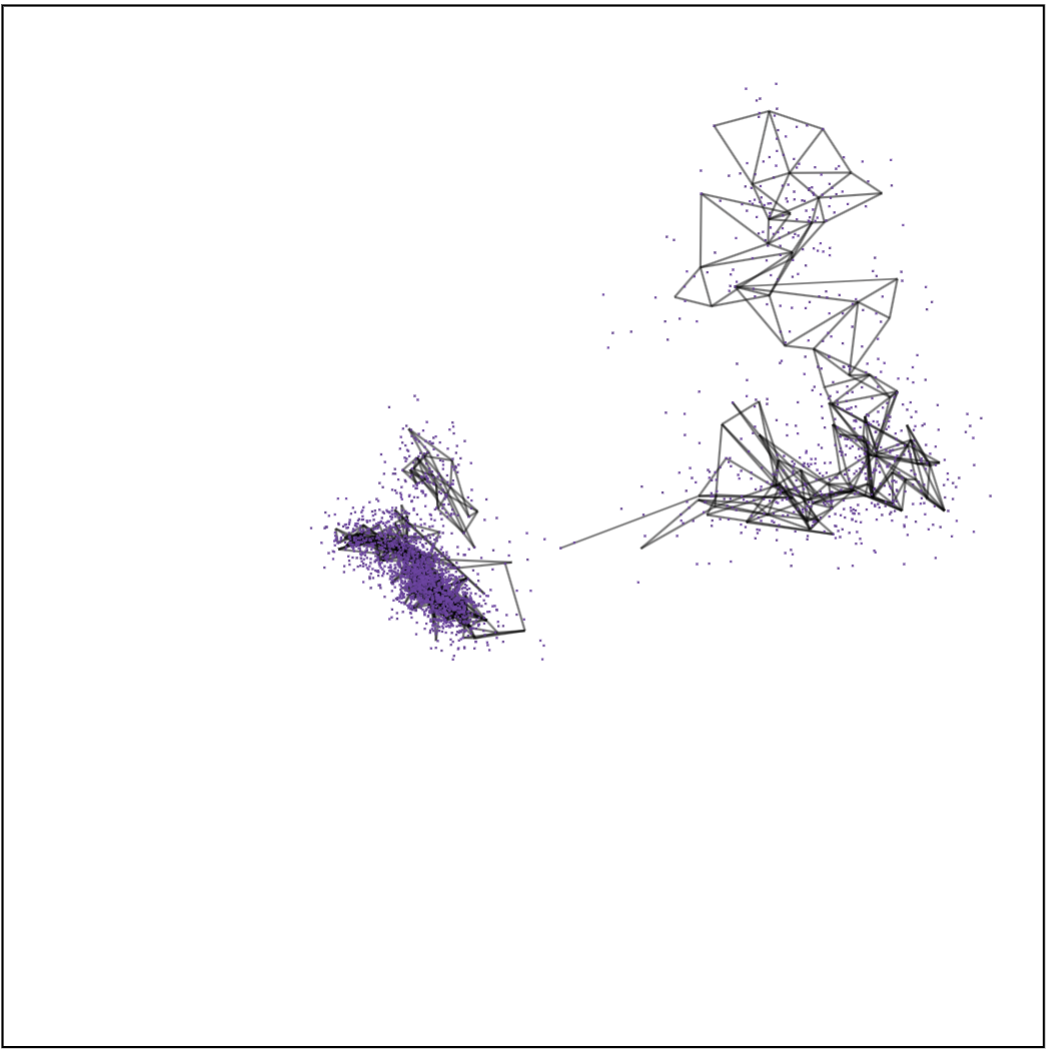
\includegraphics{figures/pbmc3k/sc_5.png}

}

\subcaption{\label{fig-pbmc2_sc5}}

\end{minipage}%
%
\begin{minipage}{0.33\linewidth}

\centering{

\captionsetup{labelsep=none}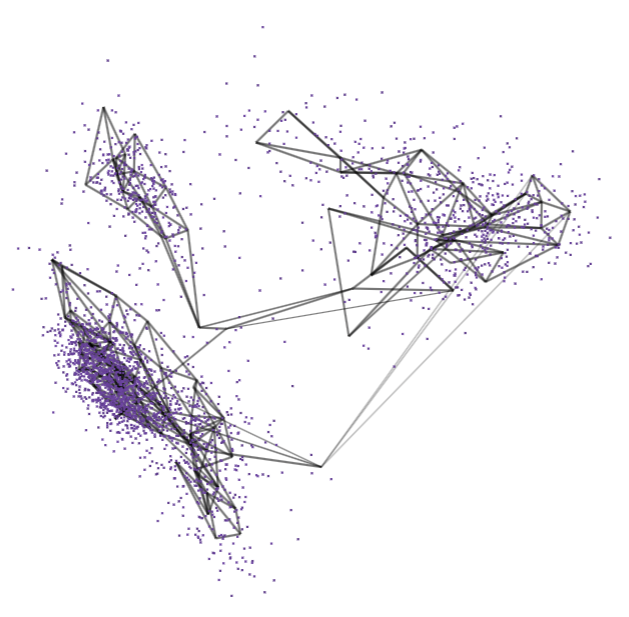
\includegraphics{figures/pbmc3k/sc_6.png}

}

\subcaption{\label{fig-pbmc2_sc6}}

\end{minipage}%

\caption{\label{fig-pbmc2_sc}Screen shots of the \textbf{langevitour} of
the PBMC3k data set, shows the model in high-D, a video of the tour
animation is available at (\url{https://youtu.be/R0EroJcGbas}).}

\end{figure}%

\subsection{digits: 1}\label{digits-1}

The MNIST dataset consists of grayscale images of handwritten digits
\citep{lecun2010}. \citet{yingfan2021} used this dataset to demonstrate
how PaCMAP preserves local structure. We selected the \gD{} embedding of
PaCMAP for the handwritten digit 1 to assess whether this is a
reasonable representation using our method. As shown in
Figure~\ref{fig-pacmap-author-img}, the angle of the digit 1 images
varies along the \gD{} structure.

\begin{figure}[H]

\centering{

\includegraphics[width=1\textwidth,height=0.22\textheight]{paper_files/figure-pdf/fig-pacmap-author-1.pdf}

}

\caption{\label{fig-pacmap-author}\(2\text{-}D\) layout from PaCMAP
applied for the digit 1 of the MNIST dataset. Is this the best
representation of the digit 1? The parameter setting is n\_components=2,
n\_neighbors=10, init=random, MN\_ratio=0.9, FP\_ratio=2.0.}

\end{figure}%

\begin{figure}[H]

\centering{

\includegraphics[width=1\textwidth,height=0.5\textheight]{paper_files/figure-pdf/fig-pacmap-author-img-1.pdf}

}

\caption{\label{fig-pacmap-author-img}Images of the handwritten digit 1
are ordered from the bottom-right to the top-left of the \(2\text{-}D\)
structure. The angle of the digit varies along this structure. Images at
the bottom-right of the \(2\text{-}D\) layout show the digit 1 angled
more to the right, while images at the top-left show the digit 1 angled
more to the left. This demonstrates how the angle changes from right to
left along the \(2\text{-}D\) structure.}

\end{figure}%

\begin{figure}[H]

\centering{

\includegraphics[width=1\textwidth,height=\textheight]{paper_files/figure-pdf/fig-model-mnist-1.pdf}

}

\caption{\label{fig-model-mnist}(a) Model generated in \(2\text{-}D\),
and (b) \(p\text{-}D\) model error in \(2\text{-}D\). The \(2\text{-}D\)
model shows a non-linear continuous structure. Most low \(p\text{-}D\)
model errors are distributed along the lower edge of the \(2\text{-}D\)
structure, while most high p-D model errors are concentrated along the
upper edge.}

\end{figure}%

According to Figure~\ref{fig-mnist1_sc1}, the non-linear continuous
structure observed in the \gD{} representation of PaCMAP (see
Figure~\ref{fig-pacmap-author}) is also visible when visualizing the
model overlaid on the data space. This indicates that PaCMAP accurately
captures the structure of the \pD{} data. Additionally, the model shows
a twisted pattern within the non-linear structure in \pD{} space (see
Figure~\ref{fig-mnist1_sc2}), which is an additional pattern not visible
in the \gD{} representation (see Figure~\ref{fig-pacmap-author}).
Furthermore, as shown in Figure~\ref{fig-mnist1_sc3}, some long edges
exist in the \pD{} space that are not recognized as long edges in the
\gD{} representation. However, PaCMAP is a \emph{good} \gD{}
representation of MNIST digit 1 data.

\begin{figure}[H]

\begin{minipage}{0.33\linewidth}

\centering{

\captionsetup{labelsep=none}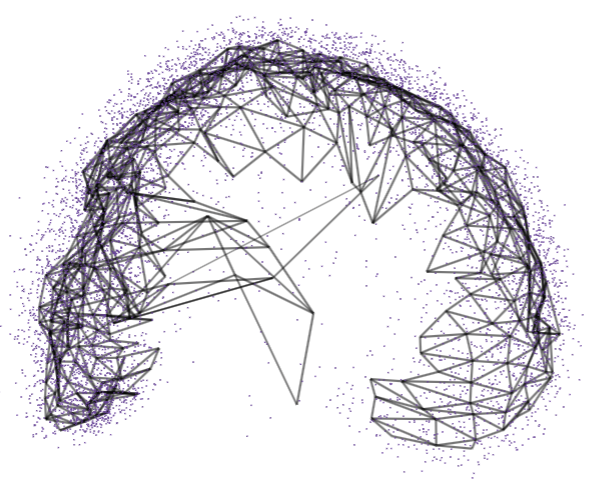
\includegraphics{figures/mnist/sc_1.png}

}

\subcaption{\label{fig-mnist1_sc1}}

\end{minipage}%
%
\begin{minipage}{0.33\linewidth}

\centering{

\captionsetup{labelsep=none}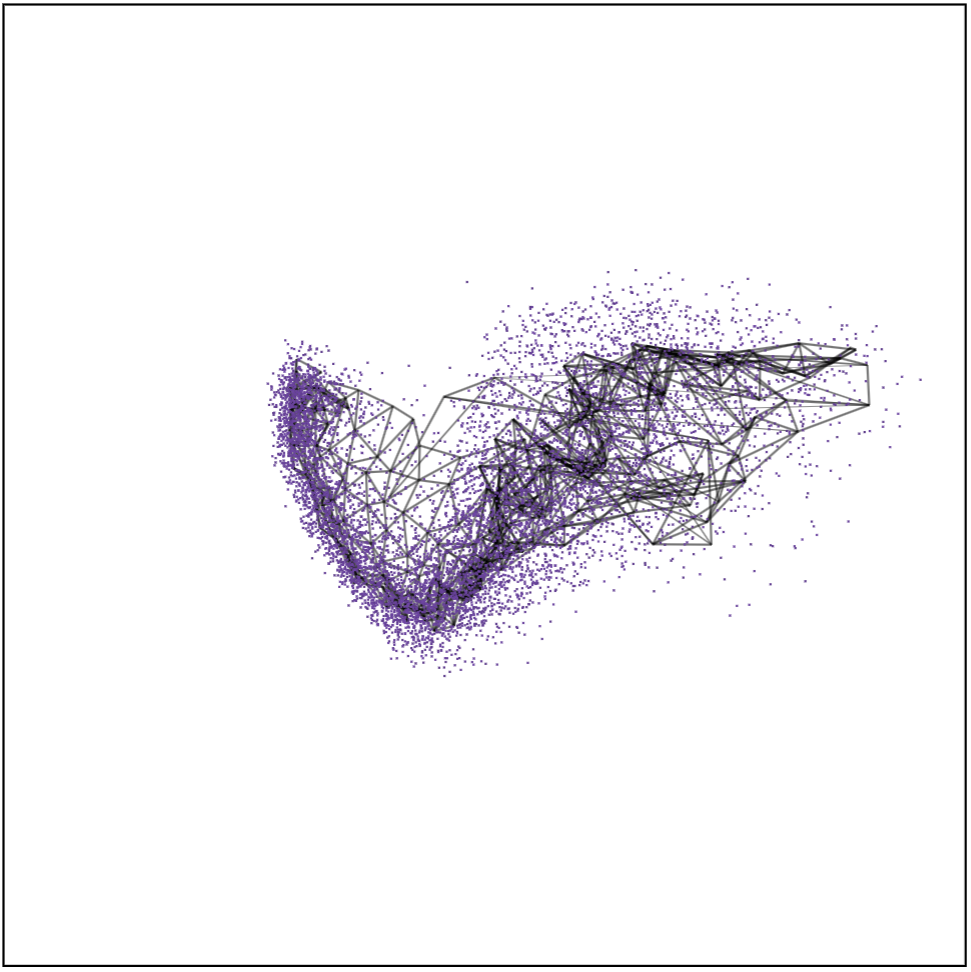
\includegraphics{figures/mnist/sc_2.png}

}

\subcaption{\label{fig-mnist1_sc2}}

\end{minipage}%
%
\begin{minipage}{0.33\linewidth}

\centering{

\captionsetup{labelsep=none}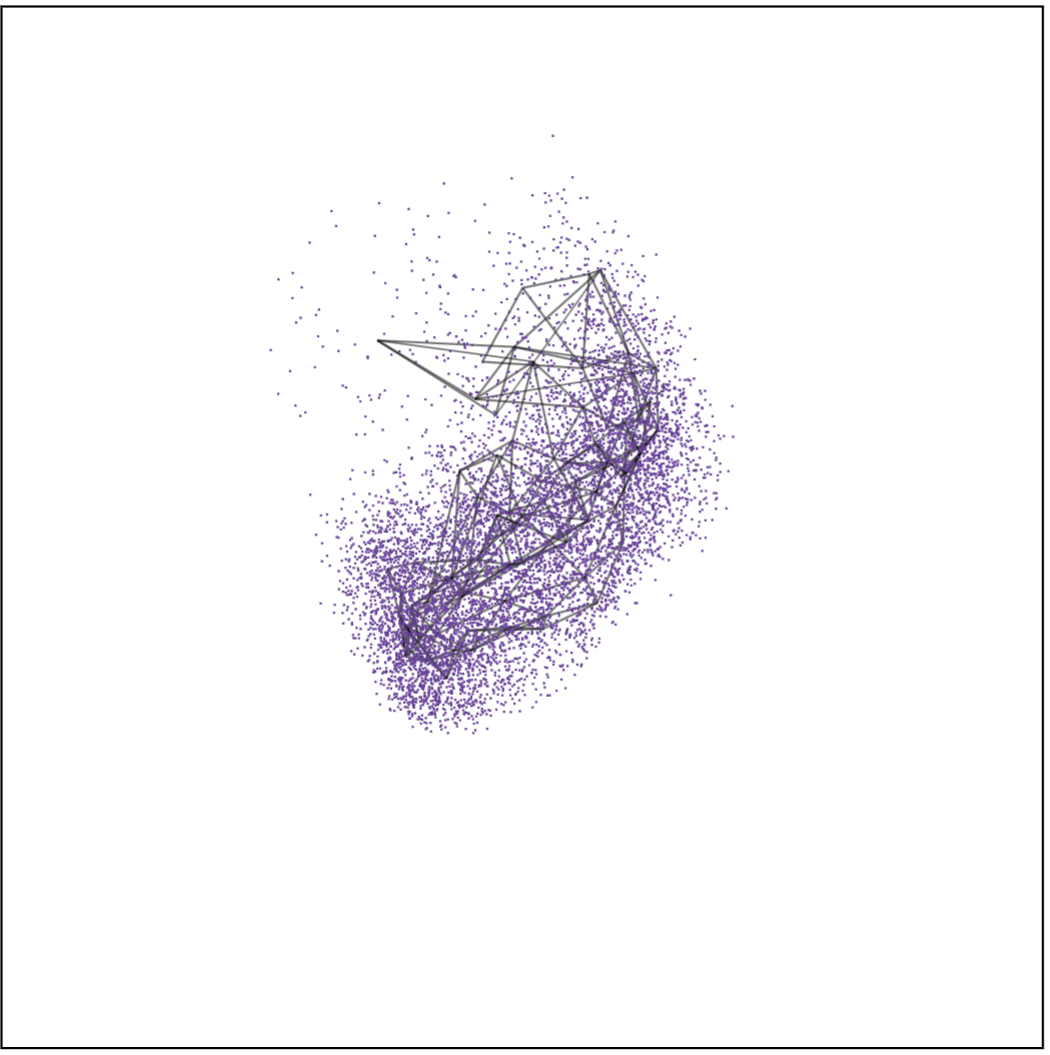
\includegraphics{figures/mnist/sc_3.png}

}

\subcaption{\label{fig-mnist1_sc3}}

\end{minipage}%

\caption{\label{fig-mnist1_sc}Screen shots of the \textbf{langevitour}
of the MNIST digit 1 data set, shows the model-in-data space, a video of
the tour animation is available at
(\url{https://youtu.be/zq2GM9qvUNA}).}

\end{figure}%

There are certain data points that exhibit high error rates due to their
deviation from the usual \pD{} data structure, which makes them
anomalies (see Figure~\ref{fig-model-mnist} (b)). These anomalies can be
classified into two types: those that are anomalies within the
non-linear structure and those that lie outside of it. The images
associated with high model error points within the non-linear structure
display different patterns of the digit 1, as shown in
Figure~\ref{fig-mnist-anomalies} (a). However, when comparing these
images to the ones found outside of the non-linear structure, it becomes
evident that the latter display different patterns of the digit 1 (see
Figure~\ref{fig-mnist-anomalies} (b)).

\begin{figure}[H]

\centering{

\includegraphics[width=1\textwidth,height=0.35\textheight]{paper_files/figure-pdf/fig-mnist-anomalies-1.pdf}

}

\caption{\label{fig-mnist-anomalies}Some images of handwritten digit 1
which occur high model error (a) within the non-linear strcuture, and
(b) outside the non-linear structure. The images shows different
patterns of digit 1.}

\end{figure}%

\section{Discussion}\label{sec-discussion}

\begin{itemize}
\tightlist
\item
  Summarise contributions
\item
  Explain where it is expected or not expected to work, eg higher
  dimensional relationships
\item
  Human behaviour, the desire to have more certainty, and a tendency to
  prefer the well-separated views
\item
  Predicting new observations in \(k\)-D
\item
  Extending layouts beyond \(k\)-D, when 2D is clearly inadequate.
\item
  Diagnostic app to explore differences in distances
\item
  What might be useful enhancements
\end{itemize}

\section*{References}\label{references}
\addcontentsline{toc}{section}{References}

\renewcommand{\bibsection}{}
\bibliography{bibliography.bib}

\newpage{}




\end{document}
